\documentclass[12pt]{article}  % 官方要求字号不小于 12 号,此处选择 12 号字体
% \linespread{1.1}
% \bibliographystyle{plain}
% 本模板不需要填写年份,以当前电脑时间自动生成
% 请在以下的方括号中填写队伍控制号
\usepackage[]{easymcm}  % 载入 EasyMCM 模板文件
\usepackage{palatino}  
\usepackage{pdfpages}
\usepackage{longtable}
\usepackage{tabu}
\usepackage{threeparttable}
\usepackage{listings}
\usepackage{paralist}
\usepackage{setspace}
\usepackage{CJKutf8}
\usepackage{textcomp} % 必须加上,否则报错
\usepackage{hyperref}
\usepackage[framed,numbered,autolinebreaks,useliterate]{mcode}    % 添加matlab代码宏

\let\itemize\compactitem
\let\enditemize\endcompactitem
\newcommand{\upcite}[1]{\textsuperscript{\textsuperscript{\cite{#1}}}}

\title{摘要} 

% 文档开始
\begin{document}
	\begin{abstract}
		\vspace{15pt}
		本报告主要探讨了救灾机器人在人机交互和远程控制平台设计中的距离特性问题。通过Unity软件搭建模拟实验平台,并收集操作人员在操作机器人“抓取”持续运动的目标救助人员时的相关数据,基于Matlab软件进行数据分析,挖掘用户潜在的操作习惯与背后的操作逻辑规律。研究表明,在机器人与目标救援人员为相遇(拦截)关系的前提下,通过摄像头远程返回影像做出抓取判断时的决策距离与待救援人员运动的速度成正相关,而与机器人移动的速度成负相关。这些发现对未来进一步改进远程救援控制平台的设计及机器人相关物理参数的优化具有重要意义。
		\vspace{5pt}
		\noindent
		
		\textbf{关键词}: 救灾机器人、人机交互、距离特性、Unity、Matlab
	\end{abstract}
	
	\maketitle  
	
	\tableofcontents
	
	\section{Introduction}
	救灾机器人是在安全生产和防灾减灾救灾过程中,执行监测预警、搜索救援、通信指挥、后勤保障、生产作业等任务,能够实现半自主或全自主控制,部分替代或完全替代人类工作的智能机器系统的总称。救灾机器人具有感知、决策、执行等特征,可提升复杂危险场景中生产和救援的效率与安全性。地震、火灾、核泄漏等事故发生时,由于事故现场环境复杂、风险因素较多,同时可能伴有次生灾害,因此现在越来越多的事故现场救援初期采用救灾机器人进行现场救援。救灾机器人的发展与应用,代表了应急管理装备现代化发展趋势,是衡量我国应急管理体系与能力现代化的重要标志。
	
	常见的火灾救灾机器人(如下图)主要由以下几个基本部分组成:
	\begin{itemize}
		\setlength{\parsep}{0ex} %段落间距
		\setlength{\topsep}{2ex} %列表到上下文的垂直距离
		\setlength{\itemsep}{1ex} %条目间距
		\item \textbf{行走机构}:用于在复杂的地表环境下行走。
		\item \textbf{影音采集机构}(如摄像头等):用于采集复杂环境下的环境信息。
		\item \textbf{机械臂}:用于远程操控执行部分操作。
	\end{itemize}

	在救灾机器人的实际使用过程中,一般通过无线通信的方式将救灾现场的影音信息远程传送给操作人员,并由操作人员对于机器人进行一系列操作,包括控制机器人的行走路径、通过机器人的机械臂进行障碍物移除、爆炸物拆除等操作,这些操作也往往通过远程控制平台实现。因此,设计一个能与机器人自身操作特性(尺寸等参数)良好契合且操作效率与精准度较高、简洁易用的远程救援控制平台是提高救援成功率的关键。
	
	在远程救援控制平台的设计过程中必不可少地需要关注到人机交互的相关问题。一个值得注意的问题是,操作人员对于救灾机器人的物理参数可能相对了解较少,特别是在只能借助于机载摄像头对周围环境进行观察的情况下,无法通过摄像头远程返回的画面精准判断机器人与目标救助人员(多为行动不便)之间的距离,从而可能会因为二者的交互失败导致目标救助人员无法通过搭乘救灾机器人实现逃生,使得救援成功率不理想,甚至可能会由于机械臂的误操作等对目标救助人员造成二次伤害,这是我们所不希望看到的。因此,希望\textbf{通过收集操作人员(用户)在模拟实验平台中操作机器人“抓取”持续运动的目标救助人员时的相关数据,分析用户的操作习惯},从而更好地指导远程救援控制平台的设计以及机器人相关物理参数与摄像头摆放位置等的改进。
	\begin{figure}[H]
		\centering
		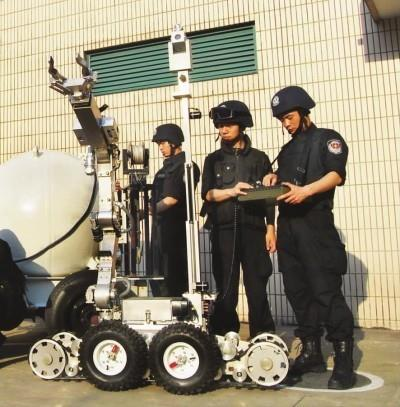
\includegraphics[width=0.3\textwidth]{1.png}
	\end{figure}
	
	\section{Literature Review}
	\begin{itemize}[$\blacktriangledown$]
		\setlength{\parsep}{0ex} %段落间距
		\setlength{\topsep}{2ex} %列表到上下文的垂直距离
		\setlength{\itemsep}{1ex} %条目间距
		\item \textbf{文献1\upcite{1}}: The different characteristics of human performance in selecting receding and approaching targets by rotating the head in a 3D virtual environment
		
		\textbf{综述}: 初始距离、目标移动速度和目标容差对于操作的准确性影响较大。初始距离会影响抓取操作的时间特性,在远离运动中,需要以高于目标速度追击目标,而靠近运动中则需要拦截目标。目标移动速度增大会增加抓取难度,特别是在远离运动中,影响更为显著。目标容差主要影响调整阶段,影响抓取精度,但不影响加速和减速阶段。
		
		\item \textbf{文献2\upcite{2}}: Beyond Fitts’s Law: A Three-Phase Model Predicts Movement Time to Position an Object in an Immersive 3D Virtual Environment
		
		\textbf{综述}: 理解距离特性对三维场景下的准确抓取来说至关重要。目标定位任务在三维虚拟环境中的特点明显不同于二维界面。例如,三维空间中的目标操作涉及大范围的手臂移动和虚拟手或射线投射技术。研究指出,人类的目标导向手臂运动包括快速的弹道阶段和慢速的修正阶段,这两个阶段在不同的因素影响下表现各异。此外,目标大小、运动幅度和目标容差是影响定位时间的主要因素,这些因素在三维环境中与传统的二维环境有所不同。
		
		\item \textbf{文献3\upcite{3}}: Capture of moving targets: a modification of Fitts' Law
		
		\textbf{综述}: 该文章主要描述了一个根据Jagacinski等人的实验数据开发的数学模型,用于描述移动目标的捕获时间。该模型在位置和速度控制系统下都经过了测试,并且与实验数据拟合良好。在移动目标下,该模型对Fitts定律的主要修改在于稳态位置误差,从而减小了有效目标宽度。在静止目标情况下,该模型退化为经典的Fitts定律。该模型预测了一个临界速度,超过这个速度目标将无法被捕获,这与Jagacinski等人的实验数据相符,可用于理解救灾机器人在不同速度下捕获目标的效率和限制。
		
		\item \textbf{文献4\upcite{4}}: 面向人机交互的机器人信息融合系统的研究与实现
		
		\textbf{综述}: 本篇文章主要探讨了在人机交互中,利用多传感器信息融合技术提升机器人对人体目标跟随的效率和精度。作者提出了一个面向人机交互的机器人信息融合系统,包括人体感知、视觉跟踪和运动跟随模块。通过运用帧间差分法和骨架验证识别人体目标,利用小波变换融合深度图像和反向投影图提高视觉跟踪精度,并采用位姿信息融合方法实现运动跟随。这些技术和系统设计有助于提升机器人在火灾场景下抓取目标救助对象的距离检测的精准性。
		
		\item \textbf{文献5\upcite{5}}: 三维虚拟空间中物体移动操作的交互模型
		
		\textbf{综述}: 这项研究通过三个实验系统探讨了影响3D空间物体移动效率的因素,并建立了相应的数学模型。研究发现,除了传统的移动距离和目标大小外,被移动物体的大小和所处深度也影响移动效率。实验结果表明,移动物体的大小影响移动过程中的加速阶段,而移动物体所处的深度则影响整体移动时间。通过以视角为单位的修正模型,研究者成功地拟合了实验数据,提高了移动操作效率的预测准确性。这一研究成果为虚拟3D空间中的人机交互设计提供了有益的参考,可为设计更有效的救灾机器人操作策略提供理论支持。
		
		\item \textbf{文献6\upcite{6}}: 虚拟运动目标人机交互方法设计与仿真
		
		\textbf{综述}: 这项研究提出了一种基于多体感融合的虚拟运动目标人机交互方法,以解决当前虚拟手型逼真度偏低的问题。利用Kinect采集深度图像和彩色图像,结合颜色直方图匹配结果,实现了对虚拟运动目标的准确识别和跟踪。通过提取目标结构信息并融合全部体感特征,构建了笛卡尔空间映射关系,以实现人机交互。仿真结果显示,该方法不仅能够获取高逼真度的虚拟手型,还能够准确跟踪和识别目标,为解决商场火灾场景下救灾机器人抓取目标救助对象的距离特性提供了实用性解决方案,使虚拟实验平台上的交互操作在现实中成为可能。
		
		\item \textbf{文献7\upcite{7}}: 救灾机器人远程操作控制台设计
		
		\textbf{综述}: 本篇文章强调了在各种灾难中,特别是火灾等复杂环境下,使用消防机器人进行救援的必要性,从消防救援的角度出发,针对地震、火灾、核泄漏等灾害提出了机器人功能需求,并结合人因工程学等相关学科知识,从宏观层面探讨了远程操作平台的构建方法,并给出了一些关键的参考数值,为实验平台的搭建提供了指导性的重要参考。
		
		\item \textbf{文献8\upcite{8}}: 可变形履带机器人数字孪生测试平台研究
		
		\textbf{综述}: 作者利用Unity引擎开展了关于多地形多运动模式矿井救灾机器人的研究,围绕虚拟空间生成崎岖巷道的数字孪生环境展开,建立了数字化描述模型,并实现了可变形履带机器人的现实层面与抽象层面的复制,构建了物理级和系统级的数字孪生样机,以及信息级的数字孪生平台。这项研究的方法和成果为类似商场火灾场景下的救灾机器人开发提供了借鉴,特别是在抓取目标救助对象的距离特性研究方面,为机器人的设计与测试提供了新思路和技术支持。
		
		\item \textbf{文献9\upcite{9}}: 一种基于三维建图和虚拟现实的人机交互系统
		
		\textbf{综述}: 该研究提出了基于三维建图和虚拟现实技术的人机交互系统,旨在提高救援机器人在商场火灾场景下的应用效率。操作人员则可通过虚拟现实系统的交互设备生成控制指令,实现对机器人的运动控制。这一系统不仅能够将机器人环境实时可视化,提供操作人员极强的沉浸感,还为人与机器人的自然交互提供了新的思路,对于促进人机交互技术的发展具有重要意义,也从技术层面为救援机器人在路径规划导航与精准定位抓取等方面提供有力支持。
		
		\item \textbf{文献10\upcite{10}}: 多模态交互中的目标选择技术
		
		\textbf{综述}: 多模态交互技术利用各种传感器捕获的信息,预测人的交互意图,提升机器对人行为的理解能力,尤其适用于目标选择任务。在人机交互系统中,目标选择任务是一项基础任务,已有多个行为模型针对多模态交互进行了描述,这些理论对于开发多模态交互技术具有指导意义,可以有效推动人机交互向更自然的方向发展,也为远程操作平台在机器人与多个目标救助人员的交互逻辑设计方面提供参考。
						
	\end{itemize}
	
	\section{Method and Results}
	在一系列对于机器人与操作平台基本需求分析的基础上,我们基于Unity软件搭建了救灾机器人远程救援模拟实验平台,并希望通过模拟实验来帮助实际平台设计进行进一步改进。落实到该实验平台,本次研究的主题可以这么描述:通过收集用户操作机器人对虚拟人实现救援过程的数据,具体而言即“救援”这一行动(平台中的交互方式表现为机器人会“抓取”待救援人员并“牵引”其共同移动到终点)中的“抓取”行为(实验中简化为用户判断并发出抓取指令与完成抓取动作过程中无延迟)发生前的瞬间机器人与待救援人员之间的距离以及两者各自的运动速度,对其进行数据分析,从而寻找彼此之间的关系。实际上,用户(即操作人员)在无任何提示的情况下,应根据摄像头回传画面中出现的待救援人员的图像来判断两者之间的距离,当用户认为距离合适时便会做出判断、发出“抓取”指令以施行救援。但这样的主观判断往往具有不确定性,很容易造成误判从而带来不必要的损失甚至是二次伤害。因此,我们希望通过模拟实验的数据分析,初步得到机器人和待救援人员的移动速度与合适的实际抓取距离之间的关系,尽可能地探索用户主观判断抓取时机的规律,从而可以在检测两者数据的情况下,推测两者与合适的实际抓取距离之间的关系,进而可以提前在用户操作平台界面以UI形式给出提示,实现更精准更快速的救援,提高救援效率;同时这样的结果也可以反馈到摄像头安装位置的确定以及机械臂长度等等物理参数的确定过程,基于人因与工效学实验的结果进一步优化整体的结构设计,使整体更易上手、提高易用性。
	
	\begin{figure}[H]
		\centering
		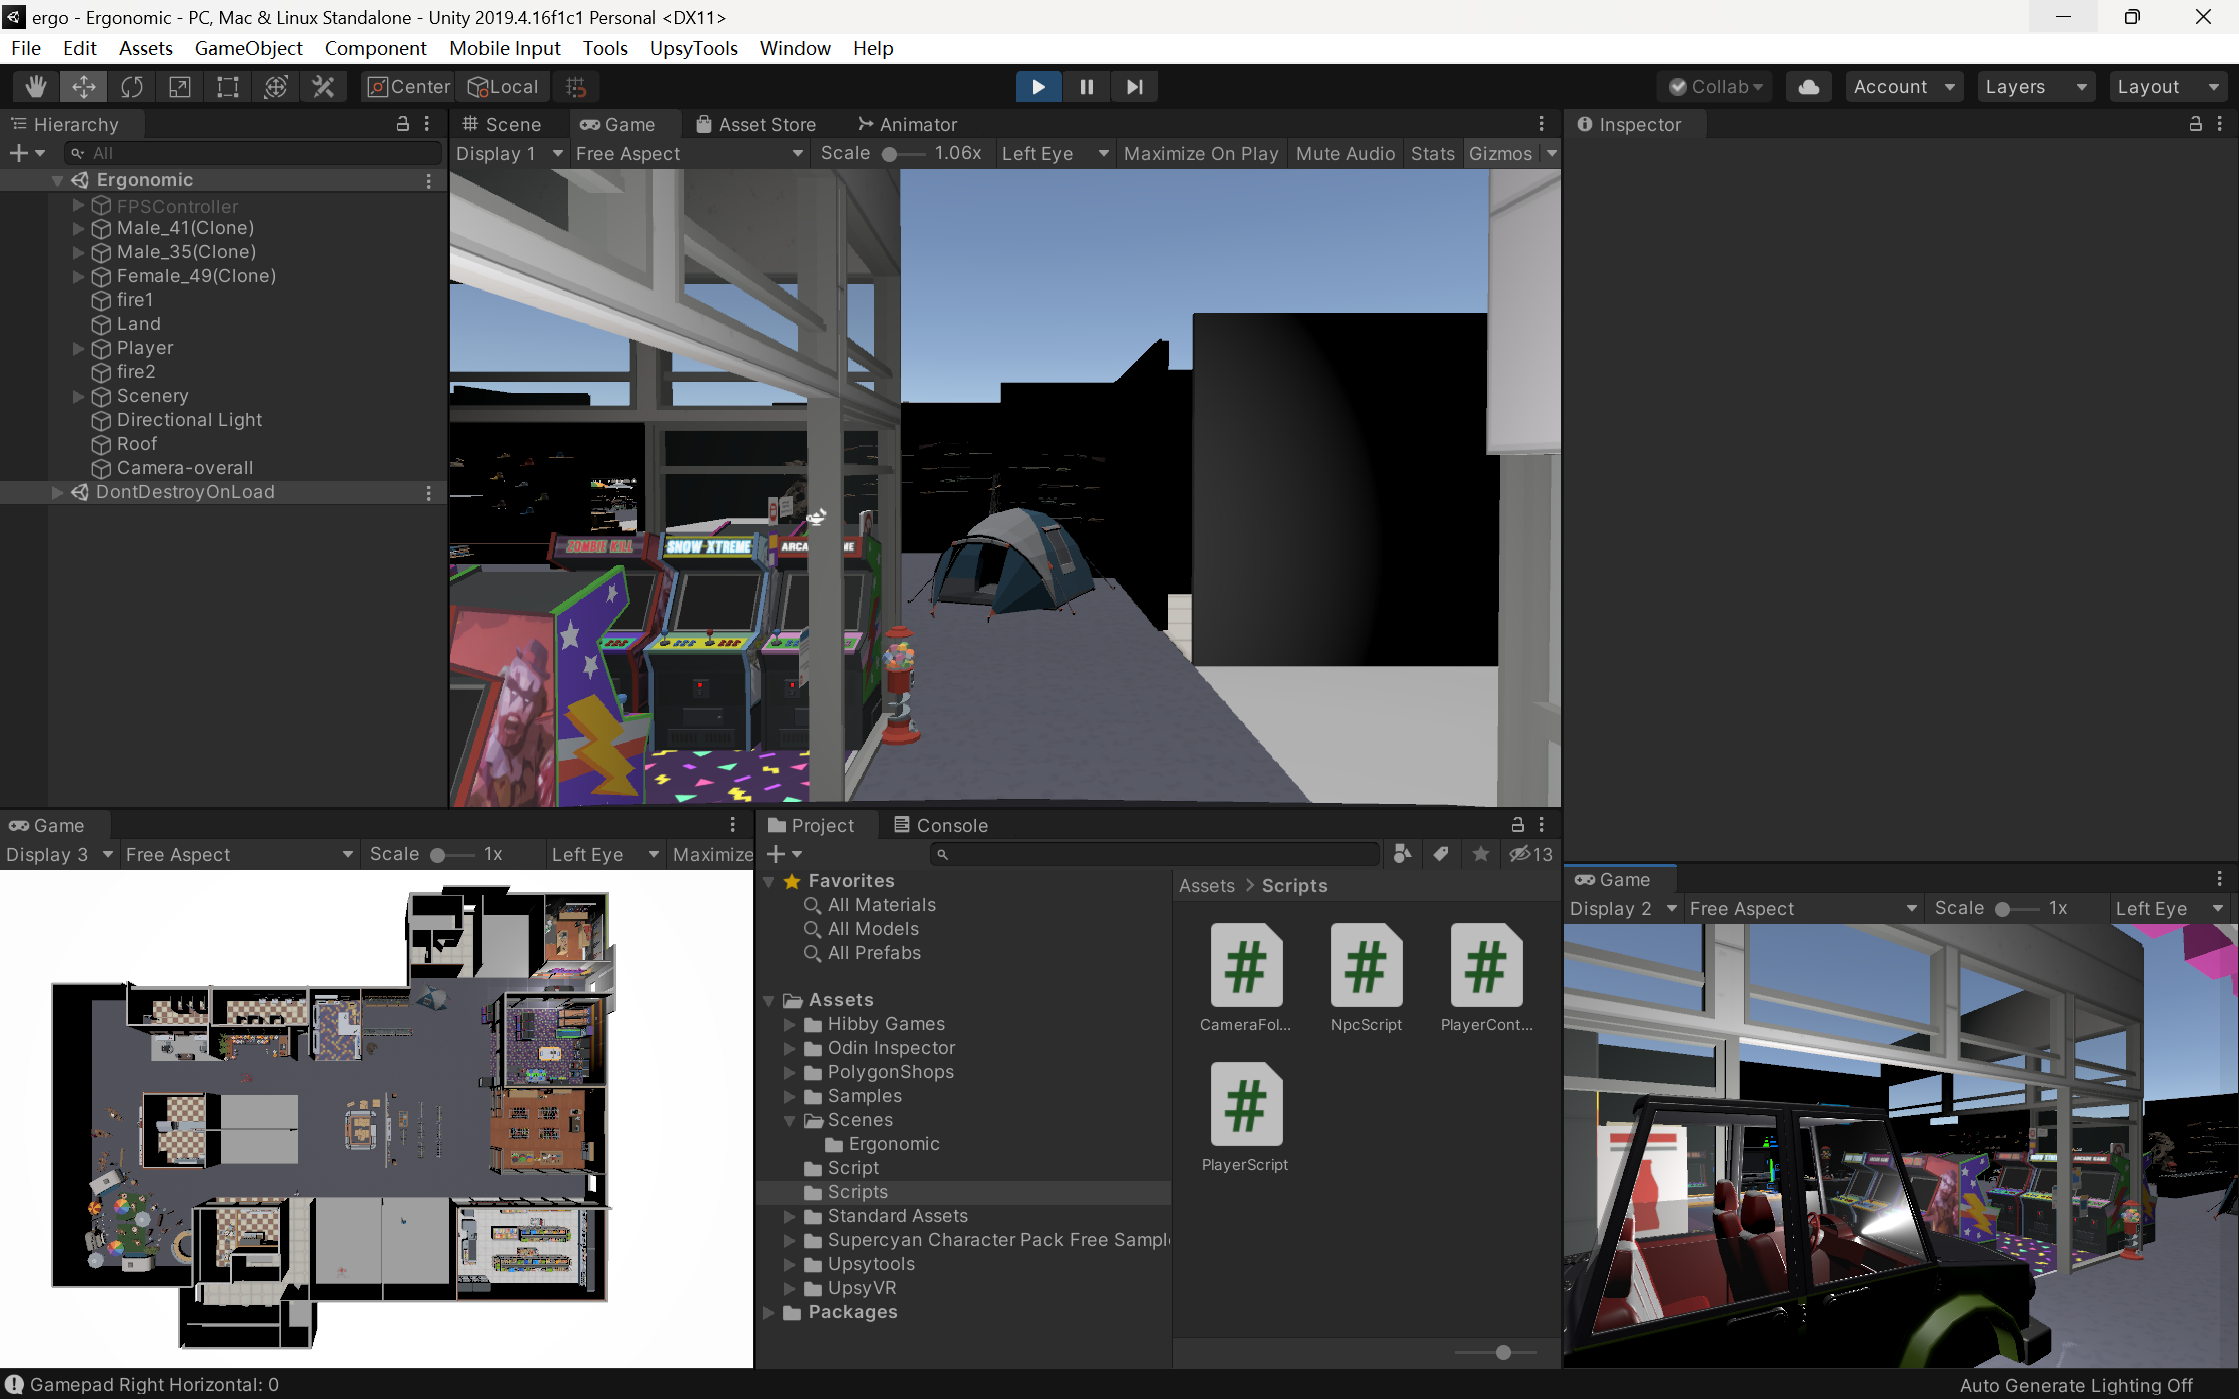
\includegraphics[width=1\textwidth]{2.png}
	\end{figure}
	
	在Unity远程救援模拟实验平台中,事先编写脚本记录所需要的实验数据,主要包括“抓取”动作发生时(按下鼠标左键即执行抓取,最大抓取范围设置为5单位)机器人与待救援人员之间的距离以及两者各自的移动速度,并编写控制与交互脚本,保证各项功能正常运行。考虑到实际应用场景,整体环境设置为商场场景,共设置3位NPC(动画与外形素材来源于蒯曙光老师的素材库\upcite{11}),各自具有不同的移动速度与行进路线;场地内模拟火灾场景,随时间推移火势会不断蔓延(烟雾扩散),在烟雾逼近时NPC会主动向最近的出口奔跑逃生,但行动不便的顾客移动速度较慢,需要机器人对其实施救援。用户(操作者)需要操作机器人,从入口出发进入火灾现场,通过“抓取”操作实施救援,最终将所有的顾客NPC全部救出至安全出口。值得注意的是,本实验仅考虑文献1\upcite{1}中的简化情形,即只考虑机器人从正面“拦截”目标;这样的假设相对是合理的,因为机器人同样是从安全出口进入商场,寻找被困人员并将其带至安全出口,基本不存在从后方“追击”被困人员的情况,且实际实验过程中在具有多视角地图的情况下(实际操作时也会将商场平面图提前导入机器人与操作平台)也没有实验者采取“绕远路”的方式实行救援。
	
	邀请到同组的5位同学作为实验者,每个人完成10次救援,共得到50组数据,并利用Matlab软件对于导出的数据集进行数据分析。原始数据集、代码与Unity实验环境均已上传至Github(链接:\href{https://github.com/Asgard-Tim/ergonomic}{https://github.com/Asgard-Tim/ergonomic}),在此仅对于数据分析过程与结果进行必要性的说明:
	
	首先,对于\textbf{抓取时刻的数据参数}进行研究,明确\textbf{自变量:机器人的移动速度$robospeed$ 、待救援人员的移动速度$humanspeed$};\textbf{因变量:两者间相距距离$distance$}。选取两者的速度作为自变量的原因是,通过摄像头画面直观进行距离判断时,除了人因规律外,还有可能对判断造成影响的就是双方的运动(类似多普勒效应),出于简化考虑这里只考虑与待救援人员“迎面相遇”的情况。对于两个不同的自变量,分别以其为横轴,两者相距距离为纵轴,绘制散点图(下左图,颜色反映另一未在坐标轴上的变量值);
	
	\begin{figure}[H]
		\centering
		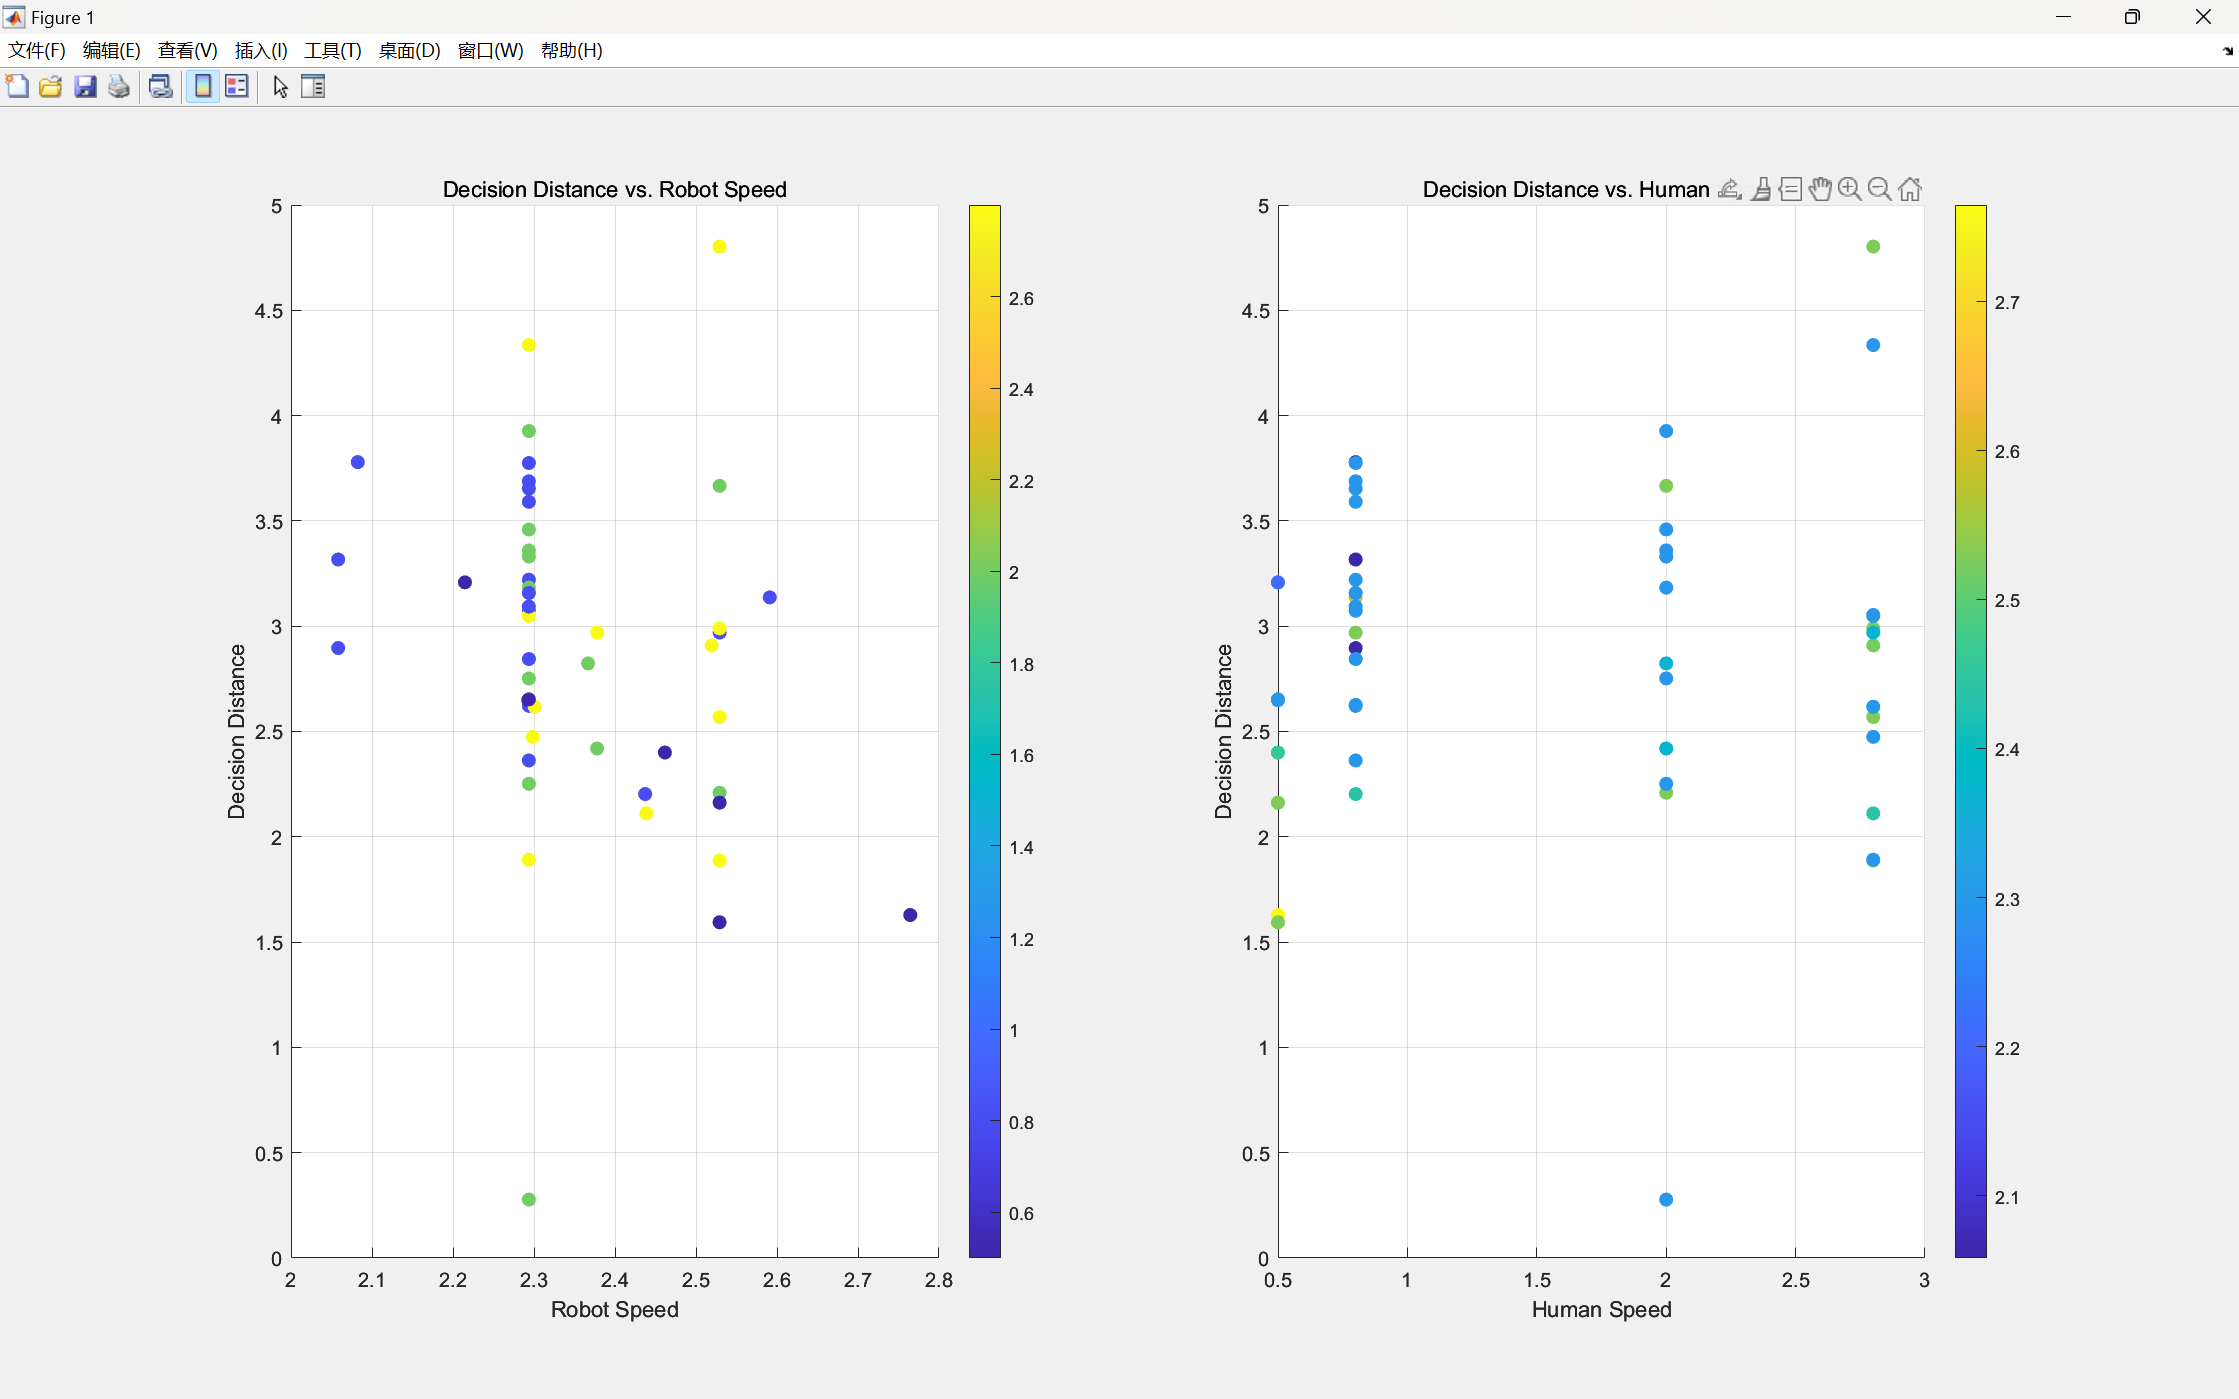
\includegraphics[width=0.45\textwidth]{3.png}
		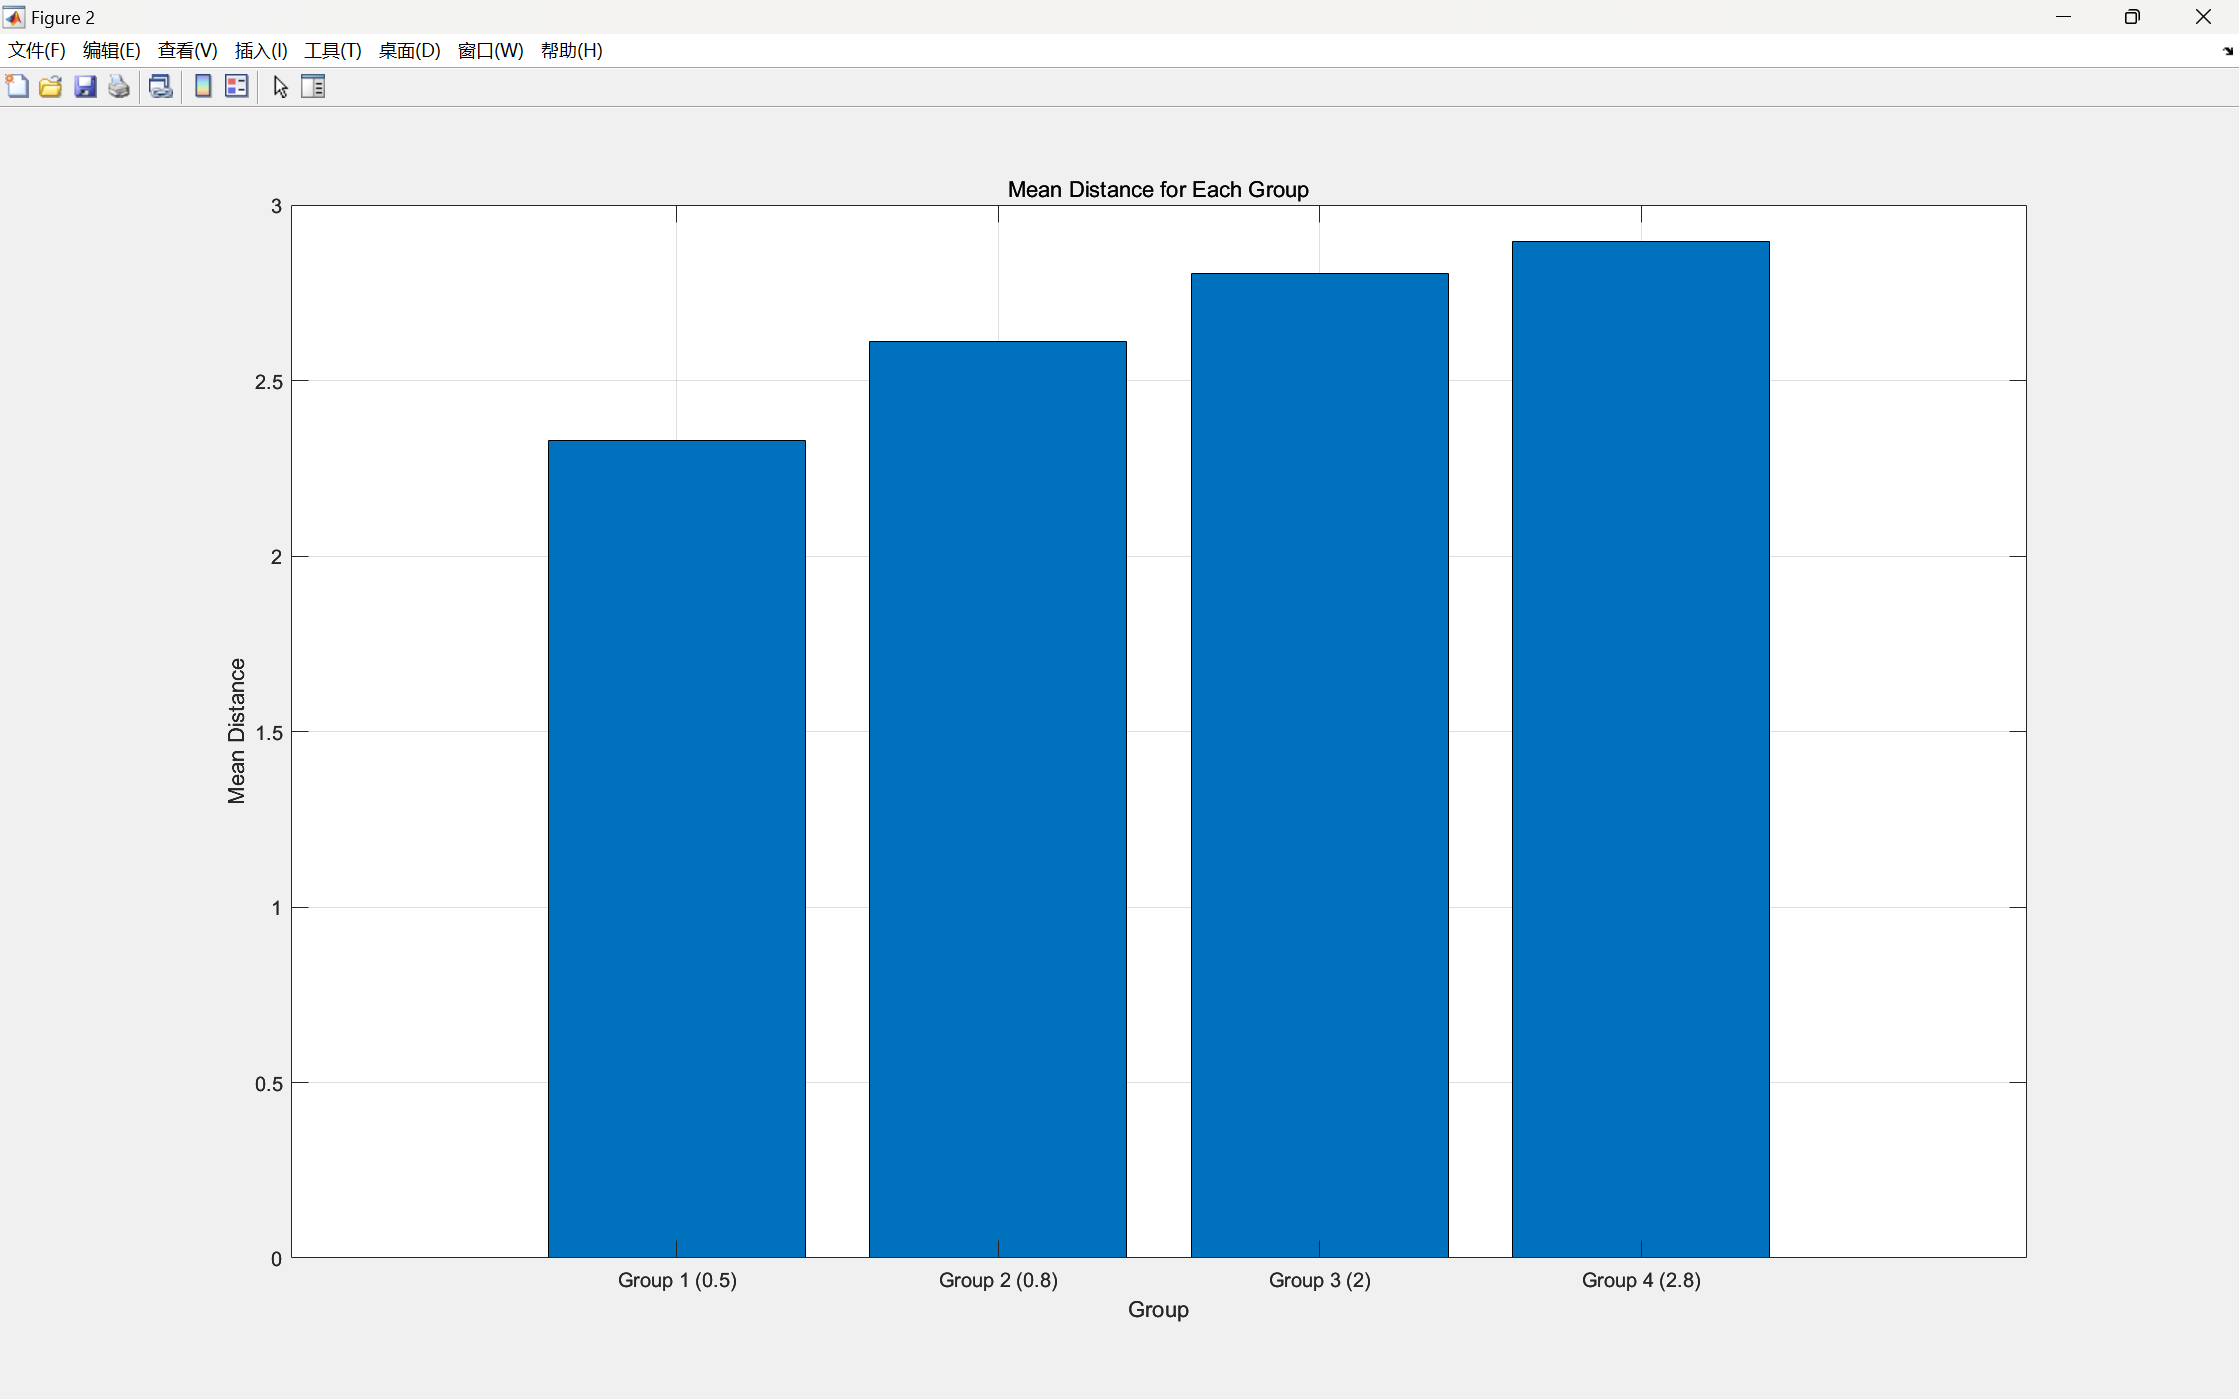
\includegraphics[width=0.45\textwidth]{4.png}
	\end{figure}
	
	可以看到,由于顾客NPC在行走与奔跑逃生时都有各自的固定设定速度,右侧以$humanspeed$为横坐标的散点图的数值点集中分布在$0.5,0.8,2.0,2.8$四处。于是,在这样四个特定的$humanspeed$聚集点上,分别对各点对应的决策距离$distance$取均值并绘制直方图观察其关于NPC移动速度$humanspeed$的变化趋势(上右图):\textbf{随着$humanspeed$ 的增加,执行“抓取”操作的决策距离$distance$也呈递增趋势}。
	
	虽然机器人的速度在实验平台中并没有以固定值的方式明确(仅设置上限为3),但是在实际操作运行中机器人的移动速度$robospeed$仍然在$2.2937$与$2.5291$两发生了大批量的聚集现象。这里的探讨分两方面进行:
	
	首先还是将聚集点用均值代替以观察总体上决策距离$distance$随机器人移动速度 $robospeed$的变化趋势(下左图);
	
	\begin{figure}[H]
		\centering
		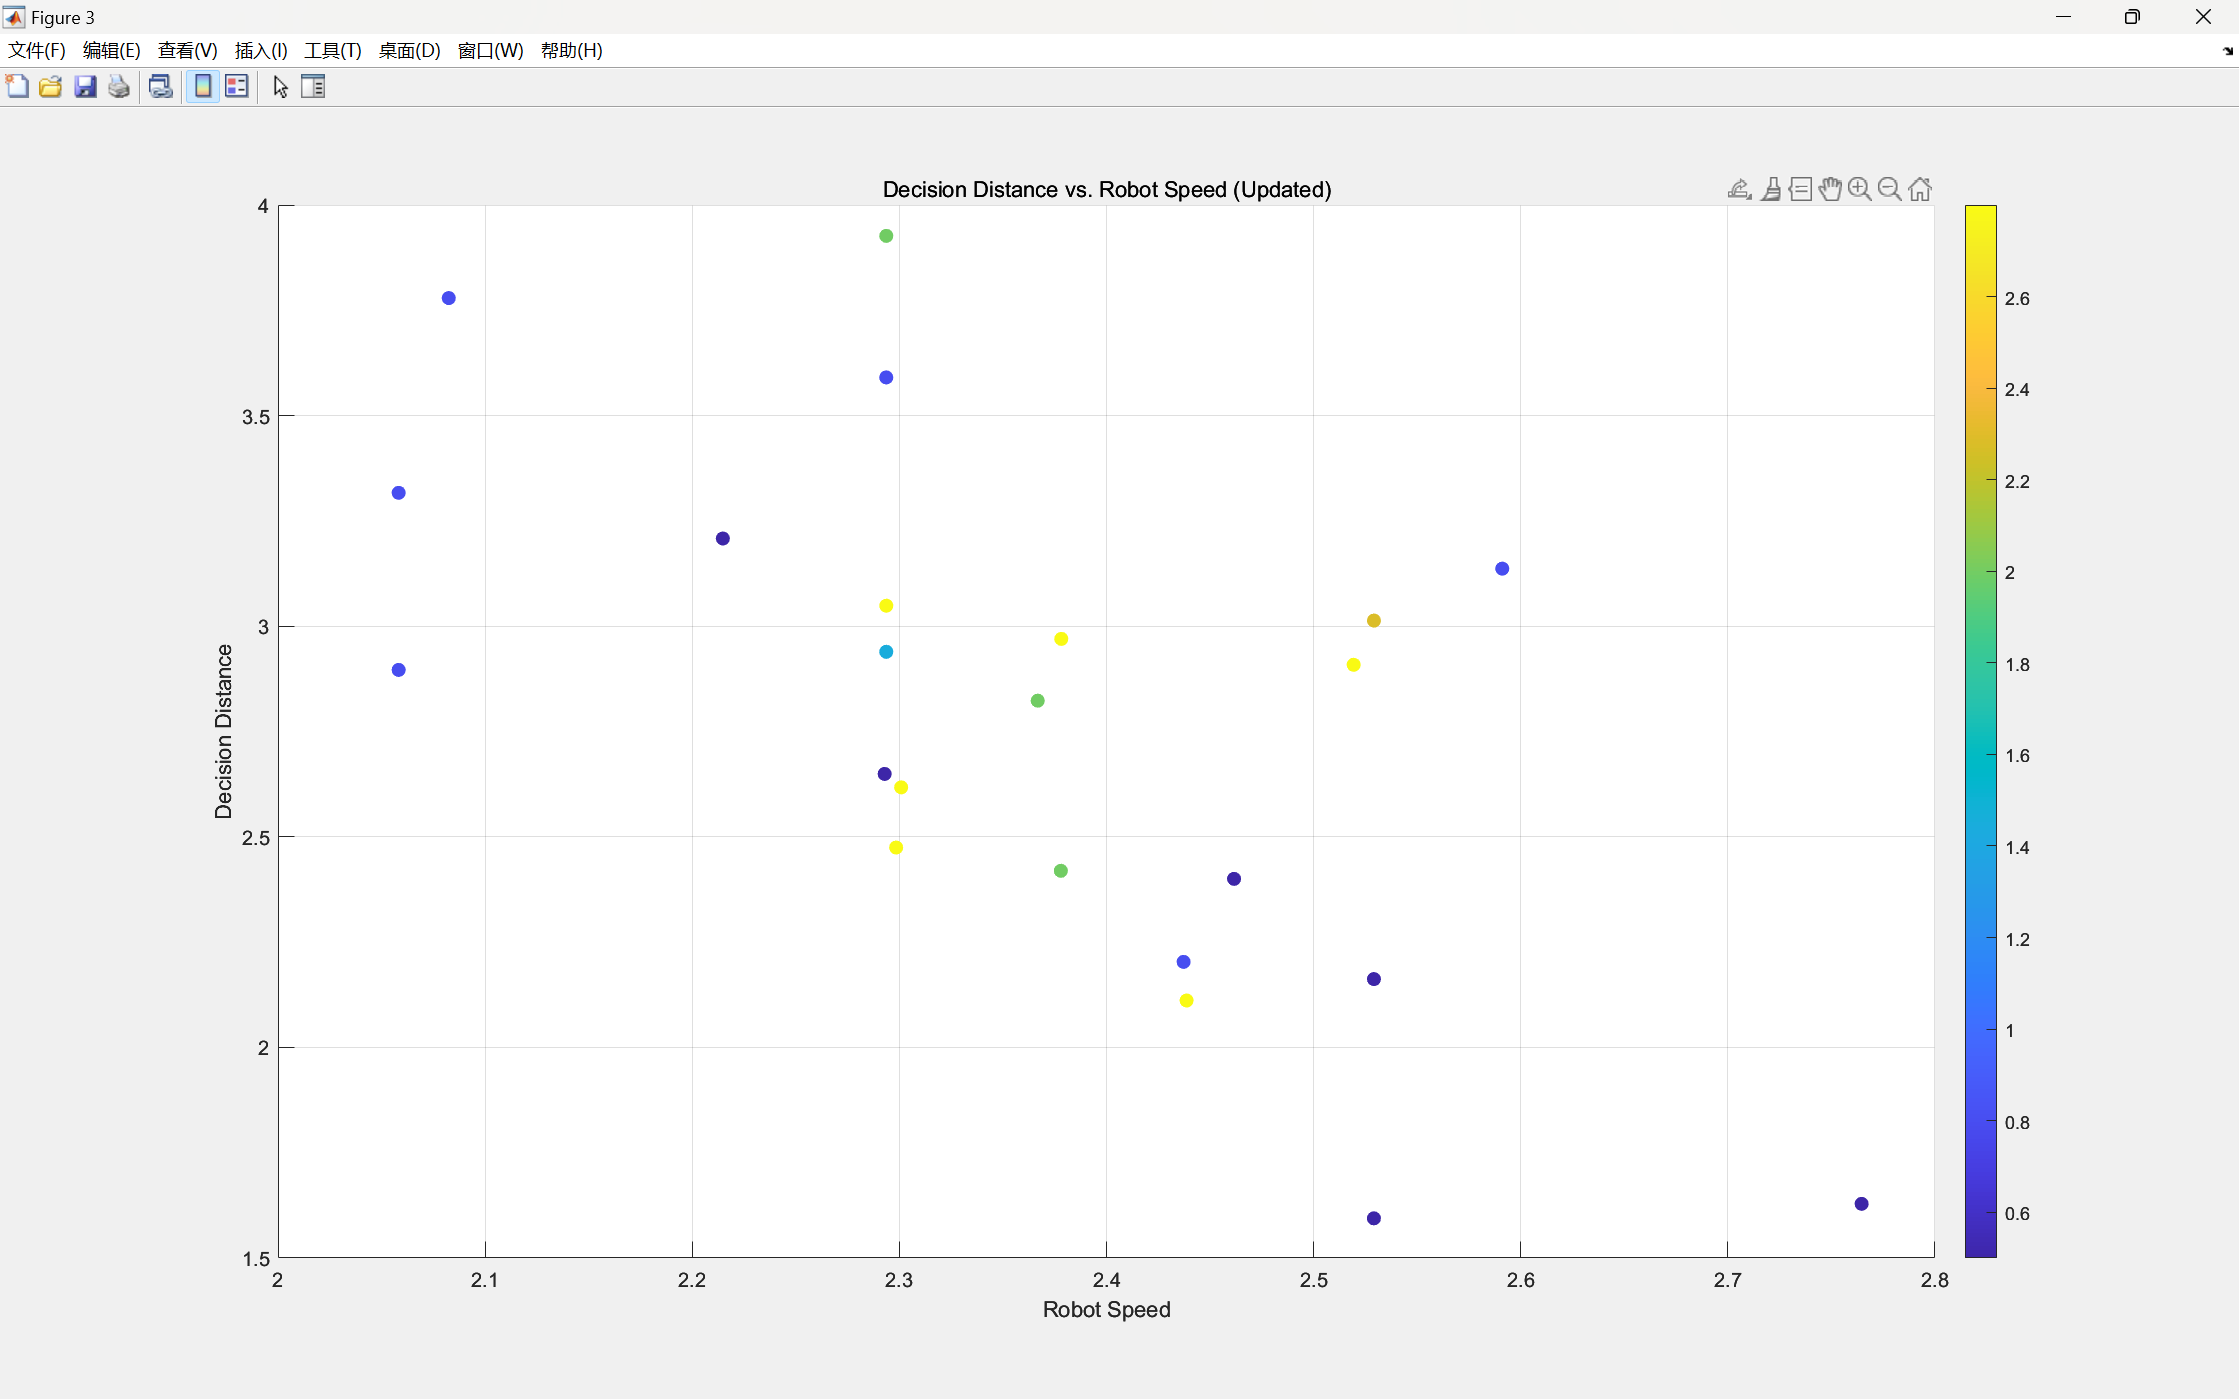
\includegraphics[width=0.45\textwidth]{5.png}
		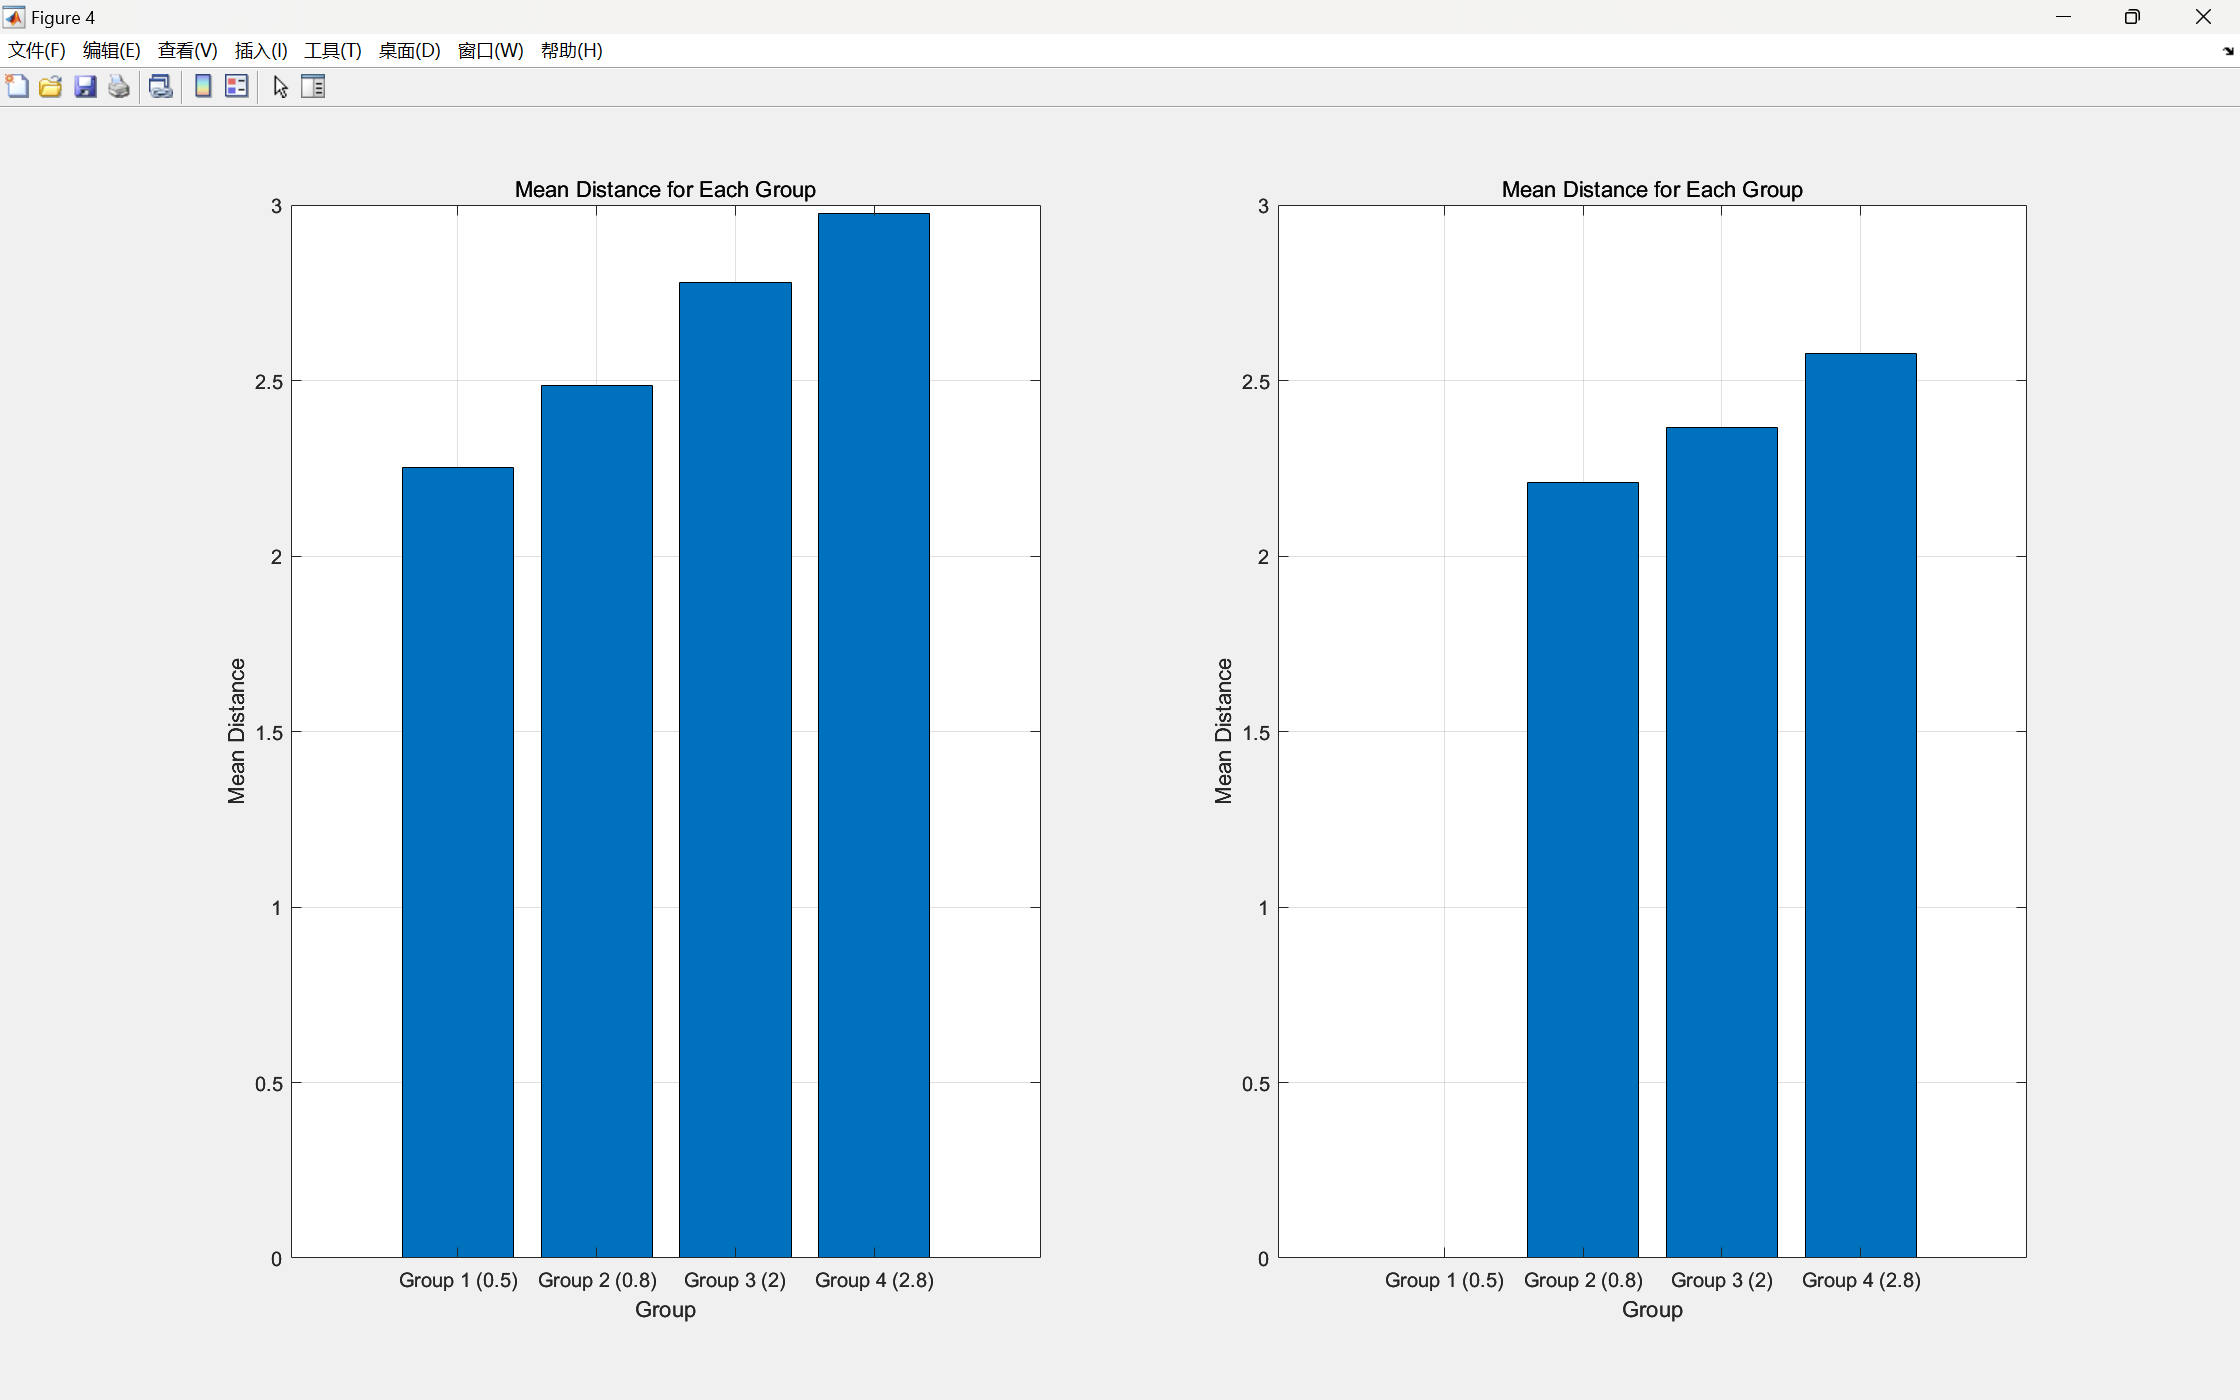
\includegraphics[width=0.45\textwidth]{6.png}
	\end{figure}
	
	尽管递减趋势较为明显,即\textbf{机器人移动速度$robospeed$应与决策距离$distance$呈负相关关系},但散点图的线性度并不好,可能是由于存在相对较大的实验误差,或是本身就不成线性关系;较为有限的样本量也导致暂时找不到较为合适的初等函数对两者关系进行拟合。
	
	另一方面,还可以对上述的数据处理过程做进一步拓展,即对于聚集点$2.2937$与 $2.5291$两处的数据可以从NPC移动速度$humanspeed$与决策距离$distance$变化关系的角度再次观测(如上右图),可以看到\textbf{在这两个聚集点处NPC移动速度$humanspeed$与决策距离$distance$仍然成正相关关系}。
	
	从总体而言,决策距离$distance$的均值为$2.8724$,NPC移动速度$humanspeed$的均值为$1.5660$,机器人移动速度$robospeed$的均值为$2.3549$。这为后续对于三者特别是决策距离的平均水平的宏观把握提供了一定的参考价值。
	
	\section{Discussion and Conclusion}
	遗憾的是,由于各方面条件限制,实验条件与样本数量有限,从50个小样本数据中很难得到更加一般化的公式层面的结果来反映用户的决策距离$distance$与两者移动速度之间的定量关系,只是从定性角度进行分析。事实上,在文献7\upcite{7}中有给出一些相应的数值参考,但并未在我们的模型上取得良好的效果;而文献2\upcite{2}、文献3\upcite{3}虽然给出了基于$Fitts' Law$的公式化的结论,但也未在我们的实验数据集上得到良好的验证。但总体而言,我们的实验数据得到的初步统计分析的结果所反映出来的变化趋势与文献中所给出的函数的趋势走向是大致一致的,即:\textbf{用户根据摄像头进行执行“抓取”操作判断的决策距离$distance$与NPC移动速度$humanspeed$成正相关,与机器人移动速度$robospeed$成负相关},这也验证了我们研究的有效性与可行性。希望能在未来能够进一步完善整个模拟操控平台、收集到更多的数据以完善统计结论,从而简化整体的交互设计,使最终实装的远程救援控制平台更加人性化、便捷、易上手,提高救援成功率,让更多的人享受科学技术带来的福祉。
	
	\newpage
	
	\begin{thebibliography}{99}
		\bibitem{1} DENG Chenglong, GENG Peng, KUAI Shuguang. (2023). The different characteristics of human performance in selecting receding and approaching targets by rotating the head in a 3D virtual environment. Acta Psychologica Sinica, 55(1), 9-21.
		\bibitem{2} Deng, C.-L., Geng, P., Hu, Y.-F., \& Kuai, S.-G. (2019). Beyond Fitts’s Law: A Three-Phase Model Predicts Movement Time to Position an Object in an Immersive 3D Virtual Environment. Human Factors, 61(6), 879-894.
		\bibitem{3} ERROL R. HOFFMANN (1991) Capture of moving targets: a modification of Fitts' Law, Ergonomics, 34:2, 211-220.
		\bibitem{4} 刘素成. 面向人机交互的机器人信息融合系统的研究与实现[D].电子科技大学,2018.
		\bibitem{5} 邓成龙,胡逸,耿鹏,等. 三维虚拟空间中物体移动操作的交互模型[C]//中国心理学会.第二十届全国心理学学术会议--心理学与国民心理健康摘要集.[出版者不详],2017:2.
		\bibitem{6} 龙年,刘智惠.虚拟运动目标人机交互方法设计与仿真[J].计算机仿真,2022,39(06):201-205.
		\bibitem{7} 于彦凤,刘力源,楚炎.救灾机器人远程操作控制台设计[J].大众标准化,2021(18):220-222.
		\bibitem{8} 魏桢. 可变形履带机器人数字孪生测试平台研究[D].中国矿业大学,2022.DOI:10.27623/d.cnki.gzkyu.2021.001514.
		\bibitem{9} 张辉,王盼,肖军浩,等.一种基于三维建图和虚拟现实的人机交互系统[J].控制与决策,2018,33(11):1975-1982.DOI:10.13195/j.kzyjc.2017.0810.
		\bibitem{10} 周小舟,宗承龙,郭一冰,等.多模态交互中的目标选择技术[J].包装工程,2022,43(04):36-44.DOI:10.19554/j.cnki.1001-3563.2022.04.004.
		\bibitem{11} Zhou, C., Han, M., Liang, Q., Hu, Y.-F., \& Kuai, S.-G. (2019). A social interaction field model accurately identifies static and dynamic social groupings. Nature Human Behaviour, 3(8), 847–855.
	\end{thebibliography}
	
\end{document} 
